%!TEX root = ../Main.tex
\section{Integer linear program formulation}
\label{s:ILP}

\begin{figure}[ht!]
\begin{center}
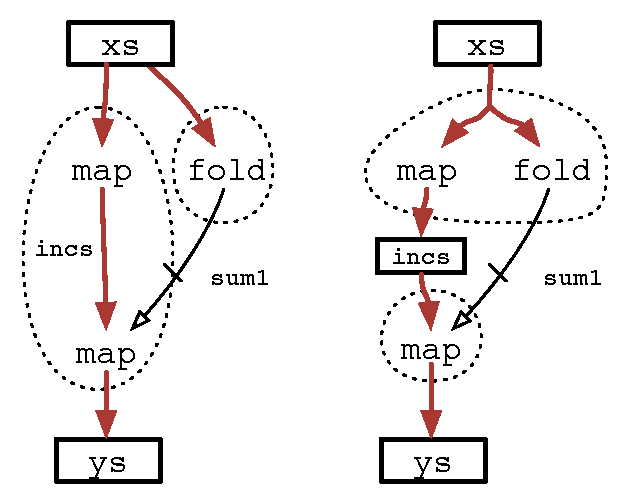
\includegraphics[scale=0.5]{figures/ex2-normalizeInc.pdf}
\end{center}
\caption{Possible clusterings for \texttt{normalizeInc}}
\label{f:normInc}
\end{figure}

The problem of finding the ``best'' clustering according to some criteria is known to be NP-hard~\cite{darte1999complexity}.
For example, in the special case of single-typed fusion, where all loops have the same iteration size, finding a clustering with the minimal number of loops can be done in polynomial time.
However, to find the minimal number of manifest arrays, each node may need to be considered in several clusters, and the problem becomes NP-hard.
Similarly, after adding multiple iteration sizes that cannot be fused together, the problem becomes NP-hard.

The clusterings of a given program are not unique; there are many valid clusterings, far too many to feasibly enumerate all of them.
There may even be multiple clusterings with the minimal number of loops. For example, consider the following program:

\begin{code}
 normalizeInc :: Array Int -> Array Int
 normalizeInc xs
  = let incs = map  (+1)    us      (A2) (B1)
        sum  = fold (+) 0   us      (A1) (B1)
        norm = map  (/ sum) incs    (A2) (B2)
    in  norm
\end{code}
For @normalizeInc@, the first option is to compute @sum@ first (@A1@), and fuse the computation of @incs@ and @norm@ into the second loop (@A2@), as shown in the first graph in Figure~\ref{f:normInc}. The other option is to fuse the computation of @incs@ and @sum@ into a single loop (indicated by @B1@), then use a second loop to compute @norm@ (indicated by @B2@). For this specific function, it is fairly obvious that Option 1 is preferable because it avoids creating the intermediate array @incs@. For large programs with many operators the optimal way to cluster operators into loops can be entirely non-obvious. 

Our objective, then, is not to simply reduce the number of loops as in~\cite{kennedy1993typedfusion}, but to reduce overall memory bandwidth, manifest arrays, and loops.
The objective of reducing manifest arrays, or maximising array contraction, has been discussed in~\cite{gao1993collective, darte2002contraction}.

In order to deal with the combinatorial explosion of potential clusterings, we describe an integer linear programming formulation.
Integer linear programming problems are defined as a set of variables, an objective linear function and a set of linear constraints.
The integer linear solver finds an assignment to the variables that minimises the objective function, while satisfying all constraints.
This problem is NP-hard, but existing ILP solvers are able to adequately solve practical problems.
Most combinator programs are small enough for this approach to be feasible, but for larger problems an approximation could be found, within a certain threshhold of the objective function.



While the different combinators are all implemented differently, certain aspects are shared between all; they operate on input arrays, use scalar variables in their worker functions, and produce output.
To simplify creation of the integer linear program formulation, we first convert a function to a dependency graph.
The dependency graph has a node for each combinator, and edges between two combinators when one uses another's output.
After the graph is created, it is converted to an integer linear program with an objective of the least memory traffic and loops, solved, and the solution converted to a clustering.

When creating the graph, it is important to note that not all loops can be fused together; firstly, loops of different size cannot be fused. Secondly, two loops cannot be fused together if an iteration in one loop relies on the output of a later iteration in another loop. For example, a @map@ may not be fused with a @fold@ if the @map@'s worker function uses the result of the @fold@.
This fusion restriction is encoded as a \emph{fusion-preventing} edge between two combinators. Other edges are \emph{fusible}, and may be fused together. If they are not fused together for whatever reason, the \emph{from} combinator must be scheduled before the \emph{to} combinator.

% The dependency graph is translated to an integer linear program. The integer linear program has some integral, boolean and real variables, an objective function to minimise, and a set of constraints that the variables must conform to. Finding a variable assignment that satisfies the constraints and is the minimal objective function is NP-hard, but existing ILP solvers tend to be sufficient for realistic problem sizes. For larger problems, we can find an approximate answer, within say $10\%$ of the optimal answer, which still gives the exact answer for small problems.


% -----------------------------------------------------------------------------
\subsection{Function $\to$ graph}
\ben{This is a different sort of graph than before. This is a dependency graph where the nodes are intermediate variables, verses the previous ``program graph'' where the nodes can also be operators. We need to contrast these properly and add a diagram of a dependency graph.}
\TODO{Put this somewhere: Fusion-preventing dependencies are akin to barrier synchronisations in the Bulk Synchronous model of parallel computation. }


Converting a function in \emph{combinator normal form} to a graph --- in fact, a DAG --- is quite simple.
Each binding becomes a node in the graph. When a binding references other arrays or scalars, there is an edge between those two nodes. Edges may be either \emph{fusible} or \emph{fusion-preventing}. Fusion-preventing edges mean that the entire input node must completely finish its execution before the output node can start executing. For example, @fold@s consume their entire input array before producing a single result, so any references to folds must be fusion-preventing. Conversely, @map@s produce output data for every input element, so may be fused.

The @gather@ operation is interesting; it takes an indices array and a data array, and for each element in indices returns that element in data.
Thus, @gather@ requires random-access in its data array, and is not fusible, but consumes indices linearly and may fuse.

\begin{tabbing}
MMMM        \= MM   \= \kill
$nodes$     \> @::@ \> $program \to V$          \\
$edges$     \> @::@ \> $program \to E$          \\
$edge$      \> @::@ \> $\{bind\} \times bind \to E$\\
\\
MMMMM       \= \kill
$nodes(bs)$ \> $= \{(name(b), \iiter_{\Gamma,C}(b)) | b \in bs\}$       \\
\end{tabbing}
Each node may simply be the name of its output binding (or bindings, in the case of @external@); as we require names to only be bound once, this is assured to be unique.
Creating edges between these nodes is simply when one binding references an earlier one. The only complication is designating edges as \emph{fusible} or \emph{fusion-preventing}.

\begin{tabbing}
MMMMM       \= \kill
$edges(bs)$ \> $= \bigcup_{b \in bs}edge(bs, b)$    \\
\\
MM             \= M \= \kill
$edge(bs, out = @fold@~f~in)$ \\
    \> $=$    \> $\{inedge(bs,out,s) | s \in fv(f)\} \cup \{inedge(bs, out, in) \}$       \\
$edge(bs, out = @map@~f~in)$  \\
    \> $=$    \> $\{inedge(bs,out,s) | s \in fv(f)\} \cup \{inedge(bs, out, in) \}$       \\
$edge(bs, out = @filter@~f~in)$  \\
    \> $=$    \> $\{inedge(bs,out,s) | s \in fv(f)\} \cup \{inedge(bs, out, in) \}$       \\
$edge(bs, out = @gather@~data~indices)$  \\
    \> $=$    \> $\{(out,data, \fusionpreventing) \} \cup \{inedge(bs, out, indices) \}$       \\
$edge(bs, out = @cross@~a~b)$            \\
    \> $=$    \> $\{inedge(bs, out, a) \}           \cup      \{(out, b, \fusionpreventing) \}$ \\
$edge(bs, outs = @external@~ins)$  \\
    \> $=$    \> $\{(outs,i, \fusionpreventing) | i \in ins \}$ \\
\\
$inedge(bs,to,from)$ \\
    \> $|$ \> $(from = @fold@~f~s) \in bs$     \\
    \> $=$ \> $(to, from, \fusionpreventing)$  \\
    \> $|$ \> $(outs = @external@ \ldots) \in bs     \wedge from \in outs$     \\
    \> $=$ \> $(to, outs, \fusionpreventing)$  \\
    \> $|$ \> $otherwise$                      \\
    \> $=$ \> $(to, from, \fusible)$            \\
\end{tabbing}


% -----------------------------------------------------------------------------
\subsection{Graph $\to$ ILP}
With the dependency graph now constructed, it must be converted to an integer linear program. The integer linear program will contain some variables, an objective function, and constraints that the variables must conform to. An external solver will find and return a variable assignment that minimises the objective function. With the variable assignment, the graph's nodes are partitioned into a clustering, and then flow fusion\cite{lippmeier2013flow} is used to extract imperative loops for each cluster.

The variables in the ILP formulation can be split into three groups:

\begin{tabbing}
M   \= MM \= MMMMMMM \= MM \= \kill
$x$   \> @:@  \> $node \times node$ \> $\to$ \> $\mathbb{B}$
\end{tabbing}
The first and most important group is created for every pair of nodes, and has a boolean value indicating whether the two nodes can be fused. If $x_{ij} = 0$, then $i$ and $j$ are fused together. While it may seem counterintuitive for 0 to mean fused and 1 unfused, it means the objective function can simply minimise a weighted $x_{ij}$, and also makes later precedence constraints simpler. The values of these variables are used to construct the partitioning at the end, such that $\forall i,j.\ x_{ij} = 0 \iff cluster(i) = cluster(j)$.
If two nodes are ``fused together'', it means that their combinators will be in the same cluster.

\begin{tabbing}
M   \= MM \= MMMMMMM \= MM \= \kill
$\pi$ \> @:@  \> $node$             \> $\to$ \> $\mathbb{R}$
\end{tabbing}
The second group of variables is used to ensure that the clustering is acyclic -- that is, there must be an ordering to execute each clusters' dependency clusters before executing the cluster itself.
For each node $i$, we associate a real $\pi_i$ such that every node $j$ after $i$ we have $\pi_j > \pi_i$. This has the effect of requiring an acyclic clustering, as if one node is after another its $\pi$ must be strictly greater than its predecessor, and the predecessor must be strictly less than the successor. If two nodes are to be fused together, their $\pi$ values must be the same.

As an example of a cyclic clustering, consider:
\begin{code}
cycle us
 = let xs  = map (+1) us          (C1)
       sum = fold xs              (C2)
       zs  = map (+sum) xs        (C1)
\end{code}
There is no fusion-preventing edge directly between @xs@ and @zs@, but there is a fusion-preventing edge between @sum@ and @zs@.
If @xs@ and @zs@ were clustered together in @C1@ and @sum@ were in cluster @C2@, there would be a dependency cycle between @C1@ and @C2@, and neither could be executed before the other.

\begin{tabbing}
M   \= MM \= MMMMMMM \= MM \= \kill
$c$   \> @:@  \> $node$             \> $\to$ \> $\mathbb{B}$
\end{tabbing}
The third, and final, group of variables are purely for minimisation, indicating whether a node's array is \emph{fully contracted}.
They are not required for correctness of the clustering, but are used in the objective function.
A node's array will be fully contracted --- that is, it will be replaced by a scalar --- if all nodes that use this array are fused together: $c_i = 0 \iff \forall (i',j) \in E.\ i = i' \implies x_{ij} = 0$.


% -----------------------------------------------------------------------------
\subsubsection{Unoptimised version}
Before showing the optimised version with certain constraints removed (\S\ref{s:OptimisedConstraints}), this simpler, unoptimised version is shown.
The only difference is that fewer constraints and variables are required in the optimised version, but both versions give the same clustering.
This unoptimised version generates clustering constraints and variables for every pair of nodes, regardless of whether they may, in fact, be fused together.
Later, we show that certain constraints and variables can be removed when there is a fusion-preventing edge between two nodes.


\paragraph{Acyclic and precedence-preserving}

\begin{tabbing}
MMMMM   \= MMM \= M \= MMM \= M \= MMM \= \kill
Minimise   \> \ldots \\
Subject to \> \ldots \\
           \>    $x_{ij}$ \> $\le$ \> $\pi_j - \pi_i$ \> $\le$ \> $N x_{ij}$ \\
           \>             (an edge from $i$ to $j$)            \\
           \> $-N x_{ij}$ \> $\le$ \> $\pi_j - \pi_i$ \> $\le$ \> $N x_{ij}$ \\
           \>             (no edge from $i$ to $j$)            \\
           \> \ldots
\end{tabbing}
As per Megiddo\cite{megiddo1998optimal}, we look at every pair of nodes $i$ and $j$.

Whether there is an edge between $i$ and $j$ or not, if the two are fused together, then $x_{ij} = 0$. If $x_{ij} = 0$, then both cases may be simplified to $0 \le \pi_j - \pi_i \le 0$, which is equivalent to $\pi_i = \pi_j$. \ben{Highlight that ``fused together'' means ``in the same cluster'', and that operators can be fused even if there are no direct edges between them.}

Otherwise, if the two nodes are not fused together, then $x_{ij} = 1$. If there is an edge between $i$ and $j$, the constraint simplifies to $1 \le \pi_j - \pi_i \le N$, where $N$ is the number of nodes in the graph. This constraint means that the difference between the two $\pi$s must be at least 1, and less than $N$. Since there are $N$ nodes, the maximum difference between any two $\pi$s would be at most $N$, so the upper bound of $N$ is large enough to be safely ignored. This means the constraint can roughly be translated to $\pi_i < \pi_j$, which enforces the acyclic constraint.

If there is no edge between $i$ and $j$ and the two are not fused together, then $x_{ij} = 1$ and the constraint simplifies to $-N \le \pi_j - \pi_i \le N$, which effectively puts no constraint on the $\pi$ values.
Note, however, that other edges may still constrain $i$ or $j$.


\paragraph{Fusion-preventing edges}
\begin{tabbing}
MMMMM   \= MMM \= M \= MMM \= M \= MMM \= \kill
Minimise   \> \ldots \\
Subject to \> \ldots \\
           \> $x_{ij}$    \> $=$   \> $1$             \>       \>            \\
           \> (fusion-preventing edges from $i$ to $j$)      \\
           \> \ldots
\end{tabbing}
As per Megiddo\cite{megiddo1998optimal}, for every fusion-preventing edge, we add the constraint $x_{ij} = 1$, so that no fusion can occur. This, together with the precedence constraints above, has the effect of enforcing $\pi_i < \pi_j$.


\paragraph{Fusion between different iteration sizes}

\begin{tabbing}
MMMMM   \= MMM \= M \= MMM \= M \= MMM \= \kill
Minimise   \> \ldots \\
Subject to \> \ldots \\
           \> $x_{ij}$    \> $=$   \> $1$             \>       \>            \\
           \> (if $\iiter_{\Gamma,C}(i) \not= \iiter_{\Gamma,C}(j) \wedge parents(i,j) = \emptyset$)  \\
           \\
           \> $x_{ij}$    \> $=$   \> $1$             \>       \>            \\
           \> (if $\bot \in \{\iiter_{\Gamma,C}(i), \iiter_{\Gamma,C}(j)\}$)  \\
           \\
           \> $x_{i'j}$   \> $\le$ \> $x_{ij}$        \>       \>            \\
           \> $x_{ij'}$   \> $\le$ \> $x_{ij}$        \>       \>            \\
           \> $x_{i'j'}$   \> $\le$ \> $x_{ij}$        \>       \>            \\
           \> (if $\iiter_{\Gamma,C}(i) \not= \iiter_{\Gamma,C}(j) \wedge parents(i,j) = \{i',j'\}$) \\
           \> \ldots
\end{tabbing}
If two nodes have different iteration sizes, they may not necessarily be fused.
If either of the nodes have no iteration size --- in which case, they are @external@ computations --- they may not be fused at all.
However, if they have parent transducers of the same size, they may be fused if both their parents are fused together, and each is fused with its respective parent.

This is the main difference to existing integer linear programming solutions: we allow nodes with different iteration sizes to be fused together, when their parent transducers are fused together.
This is an important feature for combinator-based programming, where size-changing operations such as @filter@ are used frequently.
\ben{Highlight why we want to allow this sort of fusion, and why it is specific to data flow fusion.}

As a degenerate example, consider fusing an operation on filtered data with its generating filter:
\begin{code}
 sum1 = fold (+) 0  us
 gts  = filter (>0) us
 sum2 = fold (+) 0  gts
\end{code}
Here, $parents(gts,sum2) = \{gts, gts\}$.
This generates spurious, but still valid, constraints that $gts$ must be fused with $gts$ and $gts$ must be fused with $sum2$, in order for $gts$ and $sum2$ to be fused together.
While these constraints are unnecessary in this case, they are harmless.

In the same example, $sum1$ and $sum2$ also have different iteration sizes.
We have that $parents(sum1,sum2) = \{sum1, gts\}$.
This means that $sum1$ and $sum2$ may only be fused if $sum1$ is fused with $sum1$ (trivial), $sum2$ is fused with $gts$, and $sum1$ is fused with $gts$.
While it may seem like these constraints should be implied by transitivity of clustering, all clustering variables are used for the objective function.


\paragraph{Array contraction}
\begin{tabbing}
MMMMM   \= MMM \= M \= MMM \= M \= MMM \= \kill
Minimise   \> \ldots \\
Subject to \> \ldots \\
           \> $x_{ij}$    \> $\le$ \> $c_i$           \>       \>            \\
           \> (for all edges from i)            \\
           \> \ldots \\
\end{tabbing}
As per Darte's work on optimising for array contraction\cite{darte2002contraction}, we define a variable $c_i$ for each array.
An array is fully contracted if all its output edges are fused with it.
Thus, $c_i=0$ only if $\forall (i',j) \in E.\ i = i' \implies x_{ij} = 0$.
By minimising $c_i$ in the objective function, we favour solutions that reduce the number of required intermediate arrays.

If an array is fully contracted, it means that the array does not need to be materialised in memory, and can simply be replaced by a scalar variable for the current element. Contracting arrays reduces memory traffic and can reduce overall memory usage.


% -----------------------------------------------------------------------------
\subsubsection{The objective function}
\label{s:ObjectiveFunction}

To find the objective function, note that fusing loops can have three main benefits:
\begin{itemize}
\item
reducing memory traffic, such as multiple loops reading from the same array;
\item
removing intermediate arrays, thus reducing the amount of memory required;
\item
and reducing loop overhead, such as when two loops operate on different arrays of the same size.
\end{itemize}
However, these benefits cannot be considered in isolation; for example, fusing two loops to reduce loop overhead may remove potential fusion opportunities that reduce memory traffic.
When operating on large arrays that do not fit in cache, memory traffic dominates execution time.
An excessive number of intermediate arrays can also cause issues if all are live in memory at once, potentially leading to \emph{thrashing}.
The benefits of removing loop overhead are least of all; it should be performed if possible, but must never remove opportunities for other fusion. \TODO{Refer to example code that demonstrates these different opportunities.}

This total ordering can be encoded into an ILP objective function as weights.
If the program graph contains $N$ combinators, then there are at most $N$ opportunities for fusion.
The encoding of loop overhead is weight $1$, removing intermediate arrays is weight $N$, and reducing memory traffic is weight $N^2$.
This ensures that no amount of loop overhead reduction can outweigh the benefit of removing an intermediate array,
and likewise no number of removed intermediate arrays can outweigh a reduction in memory traffic.
Although, it is worth noting that reducing memory traffic does \emph{tend} to remove intermediate arrays, and vice versa.

\begin{tabbing}
MMMMM   \= MMMM \= M \= \kill
Minimise   \>     \> $\Sigma_{(i,j) \in E} W_{ij} x_{ij}$   \\
           \> \> \> (memory traffic and loop overhead)         \\
           \> $+$ \> $\Sigma_{i \in V} N c_i$  \\
           \> \> \> (removing intermediate arrays)         \\
Subject to \> \ldots                                \\
Where      \>                                       \\
           \> $W_{ij} = N^2$ \> $~|$ \> $(i,j) \in E $         \\
           \> \> \> (fusing $i$ and $j$ will reduce memory traffic)         \\
           \> $W_{ij} = N^2$ \> $~|$ \> $\exists k. (k,i) \in E \wedge (k,j) \in E $     \\
           \> \> \> ($i$ and $j$ share an input array)                                         \\
           \> $W_{ij} = 1$   \> $~|$ \> $@otherwise@$                                                  \\
           \> \> \> (the only benefit is loop overhead)                                        \\
           \\
           \> $N = |V|$
\end{tabbing}


\subsubsection{A note on transitivity}
It may seem that we could generate far fewer constraints and rely on transitivity of clustering equality $x_{ij}$.
This means that for each pair $i,j$ we wouldn't generate an $x_{ij}$ and thus not generate those constraints, unless $i$ or $j$ is a @filter@, or arc between $i$ and $j$.
This would help, but also means we can't \emph{minimise} on these removed $x_{ij}$, so the solution won't count the (rather smaller) benefits of fusing two non-connected nodes.

\subsubsection{Fusion-preventing path optimisation}
\label{s:OptimisedConstraints}
We can remove certain constraints and variables, by only checking nodes if there is no \emph{fusion-preventing path} between $i$ and $j$.
If there is a fusion-preventing path between two nodes, they are known to be in different clusters.
With our specific knowledge of the problem domain, we can simplify the integer linear program and make the job of the ILP solver easier by omitting these constraints.
Creating fewer constraints and variables should make it faster for the ILP solver to find a solution.

For the graph, we define a function $split(a,b)$ to check whether there exists a fusion-preventing path between two nodes, $a$ and $b$.

\begin{tabbing}
MMM      \= MM   \=  MMMMMMMMMMMM    \=  \kill
$split$     \> @::@ \> $name \times name \to \mathbb{B}$      \\
MM        \= M    \= \kill
$split(a,b)$ \\
    \>$=$  \>$\forall p \in path(a,b) \cup path(b,a).\ \fusionpreventing \not\in p$\\
\end{tabbing}

With $split$ defined, we can refine our formulation to only generate constraints between two nodes if there is a chance they may be fused together.
The entire formulation of the integer linear program follows.

\begin{tabbing}
MMMMM   \= MMM \= M \= MMM \= M \= MMM \= \kill
Minimise   \> $\Sigma_{(i,j) \in E} W_{ij} x_{ij} + \Sigma_{i \in V} N c_i$  \\
           \> (if $split(i,j)$)         \\
Subject to \\
           \> $-N x_{ij}$ \> $\le$ \> $\pi_j - \pi_i$ \> $\le$ \> $N x_{ij}$ \\
           \> (if $split(i,j) \wedge (i,j) \not\in E \wedge (j,i) \not\in E$)            \\
\\
           \>    $x_{ij}$ \> $\le$ \> $\pi_j - \pi_i$ \> $\le$ \> $N x_{ij}$ \\
           \> (if $split(i,j) \wedge (i,j,\fusible) \in E$)     \\
\\
           \>             \>       \> $\pi_i < \pi_j$ \>       \>            \\
           \> (if $(i,j,\fusionpreventing) \in E$)    \\
\\
\\
           \> $x_{ij}$    \> $\le$ \> $c_i$           \>       \>            \\
           \> (if $split(i,j)$) \\
           \> $c_{i }$    \> $ = $ \> $ 1 $           \>       \>            \\
           \> (if $\neg(split(i,j))$) \\
\\
           \> $x_{ij}$    \> $=$   \> $1$             \>       \>            \\
           \> (if $\iiter_{\Gamma,C}(i) \not= \iiter_{\Gamma,C}(j) \wedge parents(i,j) = \emptyset$)  \\
           \\
           \> $x_{ij}$    \> $=$   \> $1$             \>       \>            \\
           \> (if $\bot \in \{\iiter_{\Gamma,C}(i), \iiter_{\Gamma,C}(j)\}$)  \\
           \\
           \> $x_{i'j}$   \> $\le$ \> $x_{ij}$        \>       \>            \\
           \> $x_{ij'}$   \> $\le$ \> $x_{ij}$        \>       \>            \\
           \> $x_{i'j'}$   \> $\le$ \> $x_{ij}$        \>       \>            \\
           \> (if $\iiter_{\Gamma,C}(i) \not= \iiter_{\Gamma,C}(j) \wedge parents(i,j) = \{i',j'\} \wedge$ \\

           \> \> $ split(i,j) \wedge split(i',j) \wedge split(i,j') \wedge split(i',j') $) \\
MMMMM   \= MMMM \= M \= \kill
Where      \>                                       \\
           \> $W_{ij} = N^2$ \> $~|$ \> $(i,j) \in E $         \\
           \> \> \> (fusing $i$ and $j$ will reduce memory traffic)         \\
           \> $W_{ij} = N^2$ \> $~|$ \> $\exists k. (k,i) \in E \wedge (k,j) \in E $     \\
           \> \> \> ($i$ and $j$ share an input array)                                         \\
           \> $W_{ij} = 1$   \> $~|$ \> $@otherwise@$                                                  \\
           \> \> \> (the only benefit is loop overhead)                                        \\
           \\
           \> $N = |V|$
\end{tabbing}

% % !!!!!!!!!!!!!!!!!!!!!!!
% I commented the \input out in section/04-ILP.tex

\subsection{Proof}
To prove correctness of our linear program formulation, we need to prove two different things.
Firstly, the formulation's constraints must always be satisfiable; that is, there must exist a variable assignment that satisfies all constraints.
This is rather simple to show, but guarantees that the linear program will always give an answer.
The next thing to show is that any produced clustering is legal: if a variable assignment satisfies the constraints, then it is a valid and legal clustering.
This means that, not only do we get \emph{an} answer, we also get the \emph{right} answer.

%!TEX root = ../Main.tex
\subsubsection{Satisfiability}
For any program $p$, there exists a trivial clustering with no fusion at all.
We can use this as the variable assignment of $ilp(p)$.
For each pair of nodes $m,n \in p$, $x_{mn} = 1$ --- no fusion is possible.
For the $\pi$ variables, we must find a topographical ordering of the nodes in $p$, which is simple since we are assured it is a dag.

\TODO{Now, prove that this assignment actually satisfies the constraints.}


\subsubsection{Soundness}
For any program $p$ and variable asignment $v$, if $v$ satisfies the constraints for $ilp(p)$, the clustering denoted by $x_{ij}$ in $v$ is legal.

For a clustering to be legal, it must satisfy three constraints:
\begin{description}
\item[Acyclic]
after merging nodes of same cluster together, the resulting graph must be a dag
\item[Precedence preserving]
if there is an edge between two nodes $i$ and $j$, and they are not merged together, then we require $\pi_j > \pi_i$
\item[Fusion preventing]
likewise, if there is a fusion-preventing edge between two nodes $i$ and $j$, then we require $\pi_j > \pi_i$, which implies that they are not merged together
\item[Type constraint]
if two nodes $i$ and $j$ are in the same cluster, then $\tau_i = \tau_j$, or if $\tau_i$ is a subtype of $\tau_j$ (or $\tau_j$ is a subtype of $\tau_i$), then the \emph{generator} for $\tau_i$ (or $\tau_j$) must also be in the same cluster as $i$ and $j$.
    \\
    \TODO Actually, let us say $x_{ij} = 0 \implies check_{ij}$

\end{description}
where
\begin{tabbing}
MMMMM      \= M \= MMMMMMM \= MM \= \kill
$check$ \> @::@  \> $array \times array$ \> $\to$ \> $\mathbb{B}$ \\
MMMMM      \= M \= MMMMMM \= MM \= \kill
$check(i, j)$     \> $|$ \> $tau_i = tau_j$ \> $=$ \> $x_{i,j} = 0$                        \\
$check(i, j)$     \> $|$ \> $i' \in gen(i) $ \> $=$ \> $x_{i',j} = 0 \wedge x_{i,i'} = 0 \wedge check(i', j)$                        \\
$check(i, j)$     \> $|$ \> $j' \in gen(j) $ \> $=$ \> $x_{i,j'} = 0 \wedge x_{j,j'} = 0 \wedge check(i, j')$                        \\
$check(i, j)$     \> $|$ \> $tau_i \not= tau_j$\> $=$ \> $\bot$
\end{tabbing}








